%%% Presentation
\section{Presentation of the Experiments}

%% Subsection Parameters
\subsection{Parameters}
Before introducing the variables (dependent and independent) of our experiments, we will discuss its parameters. The parameters are not tested individually for each scenario, instead they are pre-selected. There are three parameters in our model:

\begin{enumerate}
    \item the error threshold $\tau_{E}$
    \item the argument acceptability $aa$ of the ABUI algorithm that generates the generalizations
    \item the redundancy $r$ between the two initial contexts of the agents.
\end{enumerate}

\paragraph{Error threshold:} the error threshold is the parameter $\tau_{E}$ already presented in Section \ref{sec:DegOfErr}. Referred as ``the degree of error tolerated'' in the figures, it gives the number of examples that is required by the agents for overall pairing partial sets to be taken into account in the definition of overall pairing relations. A different error threshold is linked to every data set, as the value of the error threshold affects the number of classes available to set up disagreements.

\paragraph{Argument Acceptability:} the argument acceptability is a parameter of the ABUI algorithm that determines weather or not a generalization generated by ABUI is considered satisfying with regard to the constraints that the model was extensionally requiring of it. For instance, during the construction of a counter-argument $\alpha$, an agent builds a set of positive and negative examples that $\alpha$ should and should not cover. In this situation, the argument acceptability is the accuracy of $\alpha$ over the sets of positive and negative examples above which the ABUI algorithm considers that $\alpha$ is satisfying enough to endorse the role of a counter-argument. By default, the argument acceptability is 0.75 in our experiments, as it is the default value used in the AMAIL argumentation framework.

\paragraph{Redundancy:} the redundancy is the percentage of each agent's initial context that is shared among them. If the agents receive 60 labeled examples at the beginning of the experiment, 30 of which are in both initial context, the redundancy is $50 \%$. If the same 60 examples are the initial contexts of both agents, the redundancy is $100 \%$. The redundancy is defined by the ratio of shared examples, the label of these examples are not taken into account and two agents might have $r=100 \%$ although they do not share a single right-path association. By default, the redundancy is zero in our experiments, as it is the most complex scenario four our agents to reach mutual intelligibility over. Indeed, a redundancy of 0 indicates that no information is initially shared by the agents in the form of examples.

%% Subsection
\subsection{Variables}
\label{sec:variables}

This section presents the variables that will be found in our experiments. They are presented in two distinct categories: independent variables (IV) and dependent variables (DV).
% IV
We have four independent variables: \emph{domain}, \emph{strategy}, \emph{setup disagreements} and \emph{number of initial concepts}.
% DV
There is a total of four dependent variables: the \emph{Synchronic Agreement Ratio}(SAR), the \emph{Diachronic Agreement Ratio}(DAR), the \emph{Exchanged Examples Ratio}(EER), the \emph{Number of Expected Concepts}(NEC) and the \emph{Number of Final Concepts} (NFC).

% VI
\subsubsection{Independent Variables (IV)}

\paragraph{Domain}
% The already presented data-sets
Each domain corresponds to a different data-set. The first two domains correspond to two of the three data-sets already presented in Chapter \ref{Examples}: \emph{Zoology} and \emph{Sponges}.
% We add Soybean minus the four small classes
The remaining domain \emph{Soybean} correspond to the eponymous data-set. The Soybean data-set has 307 instances of soybean observations spread among 19 classes of soybean diseases. There are 35 categorical attributes, some nominal and some ordered.
% Domains come with a set of parameters
While the experiments always use a redundancy of $0\%$ and an argument acceptability of $0.75$, each domain has its associated error threshold.


\paragraph{Strategy}
% The two strategies
Our model is divided in two strategies: the systematic and the lazy.
% Systematic
The systematic strategy is presented in Chapter \ref{SystematicStrategy} and is a strategy that focuses on preventing any disagreement that could occur on the overall context of the two agents.
% Lazy
The lazy strategy is presented in Chapter \ref{LazyStrategy} and unlike the systematic strategy, it focuses on solving disagreements on connected sets of disagreements once the agents encounter an error in their naming game.

\paragraph{Setup Disagreements (SDC)}
While the actual number of disagreements that the two agents will encounter depends on the learning of their initial contrast sets, the disagreements that we expect the agents to solve are experimentally set up. The set up of these disagreements has already been discussed in Chapter \ref{Examples}. This set up takes two parameters: the type of disagreements (overlap, hypo/hypernymy, synonymy or homonymy) that are set up, and for each type, the number of these disagreements.

\paragraph{Number of Initial Concepts (OCC)}
The number of initial concepts is the number of categories that are present in the data-set related to the experiment's domain. For the lowest possible error threshold, one, we have 3 concepts in the \emph{Sponges} domain, 7 concepts in the \emph{Zoology} domain, and 19 concepts in the \emph{Soybean} domain. However, increasing the error threshold $\tau_{E}$ decreases the number of initial concepts that can be used, as the initial concepts should contain at least $\tau_{E}$ examples.

% VD
\subsubsection{Dependent Variables (DV)}

\paragraph{Count of Disagreements(C:type,context)} The first measure of an experiment success is the count of each type of disagreements that exist between the two agent at the beginning and at the end of an argumentation. We therefore have an initial and a final count of disagreements, for each type of disagreements: self-disagreements, overlap disagreements, hypo/hypernymy disagreements, synonymy disagreements, homonymy disagreements, indistinguishable disagreements and untranslatable disagreements. Since there is a distinction between the local and the overall disagreements, the count can be local (as one agent sees it) or overall (as the experimenter sees it). Our model stops when there is no overall disagreement detected by the agents anymore, and by extension no local disagreement either. For this reason, we always expect the final count, either local or global and for each type of disagreement, to be equal to zero. Other variables will give a more nuanced measure of our model success.

\paragraph{Synchronic Agreement Ratio (SAR)} The Synchronic Agreement Ration, or SAR, is the ratio between the of examples from the overall context that are named through a left path association with the same unique sign by both agents when presented to them, over the total number of examples in the overall context. The SAR measures how well the agents have reached mutual intelligibility. %The RSA is defined in Definition \ref{def:SAR}.

\begin{restatable}[SAR]{df}{SAR}
\label{def:SAR}
Let $A_{1}$ and $A_{2}$ be two agents, and $K1$ and $K2$ be their contrast sets. The Synchronic Agreement Ratio of the two agents is:

\[
SAR(A_{1},A_{2}) = \frac{|\{ e \in U_{O} | e \prescript{l}{K1}{\mapsto} s \wedge  e \prescript{l}{K2}{\mapsto} s \}|}{|U_{O}|} 
\]

\end{restatable}

\paragraph{Diachronic Agreement Ratio (DAR)} The Diachronic Agreement Ratio in an agent is the additive inverse of the ratio between (1) the number of pairs of examples from an agent's initial context that were in two different concepts in the initial contrast set that later are in the same concept in the final contrast set, and (2) the number of pairs of examples that were in two different concepts in the initial contrast set. The DAR is a measure of refinement that shows how well the monotonic evolution of the contrast sets have been respected through the argumentation. % The DAR is defined in Definition \ref{def:DAR}:

\begin{restatable}[DAR]{df}{DAR}
\label{def:DAR}
Let $A$ be an agent that has $K = (U,Q)$ for initial contrast set and $K' = (U',Q')$ for final contrast set. The Diachronic Agreement Ratio of $A$ is:

\[
DAR(A) = 1 - \frac{| \{e_{1},e_{2} \in U | e_{1} \prescript{l}{K}{\mapsto} s \wedge e_{2} \prescript{l}{K}{\mapsto} s  \wedge e_{1} \prescript{l}{K'}{\mapsto} s \wedge e_{2} \prescript{l}{K'}{\mapsto} s' \wedge s \neq s' \} |}{| \{e_{1},e_{2} \in U | e_{1} \prescript{l}{K'}{\mapsto} s \wedge e_{2} \prescript{l}{K'}{\mapsto} s' \wedge s \neq s' \} |}
\]

\end{restatable}

\paragraph{Exchanged Examples Ratios (EER)} The exchanged examples ratio (EER) corresponds to the number of examples that have been sent from one agent to the other through messages, divided by the number of examples in the overall context.

\paragraph{Coverage Ratio (CR)} The coverage ratio (CR) corresponds to the number of examples from the overall context that can be associated with a sign by an agent through left-path associations, divided by the number of examples in the overall context.

\paragraph{Observed Disagreements Count (ODC)} Unlike the set-up disagreements (SD), the observed disagreements (OD) are disagreements \emph{stricto-sensus}. They are the disagreements that are observed between the agents after they learned their initial contrast sets. Similarly to the set-up disagreements, we measure their types and number. The setup disagreements are unlikely to be the only disagreements found between our two agents once they learn they initial contrast sets, as they built their knowledge upon partial information on the overall context. ODs can be counted before or after the argumentation, and using either the local context of one agent or the overall context.

\paragraph{Final Disagreements Count (FDC)} The final disagreements are the disagreements found at the end of the argumentation. While their count is interesting, a number of final disagreement equals to zero is synonymous of full synchronic agreement between the agents only in scenarios where we are not accounting a degree of error. When accounting a degree of error, there can be no disagreement between the agents while the agents still associate some examples with different signs (in a proportion indexed on the error threshold that is therefore fixed).

\paragraph{Number of Expected Concepts (NEC)} The number of expected concepts represents the total number of concepts that should be expected in a contrast set that has a concept for each polylexematic class in the combined left-path associations of both agents -- which corresponds to the result of a brute force approach to the problem addressed in this thesis. Given two agents $A_{1}$ and $A_{2}$ that have respectively $m$ and $n$ concepts in their contrast sets, their maximum number of expected concept is $2^{m+n} - 1$ concepts, which corresponds to the number of possible combinations between the agents' adjunct sets minus the empty set.

\paragraph{Number of Final Concepts (NFC)} The number of final concepts, or NFC, is the number of concepts in the final contrast set of one agent. For an agent $A$ with a final contrast set $K = (U,Q)$, the NFC is equal to $|Q|$. The NFC can be measured in any of the two agents, as our protocol ensures that both agents end the argumentation with the same number of concepts in their contrast sets.

%% Elements tested
\subsection{Tested Properties}

Our model is evaluated through an array of hypotheses that are tested. There is a total of seven tested hypotheses, each one corresponding to different combinations of experiments and testing a specific trait of our model.

\begin{enumerate}
    \item \textbf{H1: Generality} Our model allows two agents to reach mutual intelligibility without creating diachronic disagreements regardless of the type or combinations of types of disagreements between these two agents.
    \item \textbf{H2: Domain Independence}: Our model allows two agents to reach mutual intelligibility without creating diachronic disagreements regardless of the domain of their overall context.
    \item \textbf{H3: Coverage Preservation} Our model allows two agents to reach mutual intelligibility without restraining the context of the agents, as the overall context of the agents should not lose examples through the argumentation.
    \item \textbf{H4: Efficiency} Our model allows two agents to reach mutual intelligibility without exchanging any significant portion of their contexts.
    \item \textbf{H5: Scalability} A linear increase of size of the overall context does not exponentially increase the number of generalizations that need to be exchanged in order for the agent to reach mutual intelligibility.
    \item \textbf{H6: Simplicity} The number of concepts in each contrast-set after that the agents have reached mutual intelligibility is the number of expected concepts NEC that can be computed before the argumentation.
    \item \textbf{H7: Paradigm Shift} The SAR and the DAR achieved by an AMAIL argumentation after an argumentation using our model is better than the SAR and DAR achieved by an AMAIL argumentation alone, while the total computation time of our model plus an AMAIL run is lesser than an AMAIL run alone.
\end{enumerate}

%%% GENERALITY
\section{Generality}

%% We test generality on different tasks over the same domain (soybean)
The hypothesis of generality postulates that both approaches of our model can resolve each possible combination of disagreements between two agents' contrast sets, increasing their SAR while keeping their perspective DAR at one. In order to test this hypothesis, we used the Soybean data set to setup variable disagreements between two agents. We counted the number of disagreements before and after argumentation, along with the SAR and the DAR. In order to evaluate this hypothesis on a great number of disagreements and combinations of disagreements, we have repeated this experiment 200 times.

% Order the types
Four types of disagreements are being setup in each experiment: overlap, hypo/hypernymies, synonymies and homonymies. These four types are randomly ordered for each experiment, and a random number of each disagreement type is selected and then setup, one type after the other. For instance, if the overlap type has been ordered first, we select a random number between 0 and the number of classes of Soybean with more than $\tau_{E}$ examples divided by three (the number of classes required to setup an overlap disagreement) and we merge as many time three random classes in order to obtain as many overlap disagreements. For each of the 200 runs of the experiment, we setup a new random arrangement of disagreements.

% The VI are the disagreements that we set up
The independent variables of this experiment are the types of disagreements that have been setup and their number (SDC). The experiment is always using the Soybean data set, an error threshold of $\tau_{E} = 5$ and an argument acceptability of $0.75$.
% The VD are the MSA, the MDA, the SC and the EEC
The main dependent variables are the SAR and the DAR, in order to measure to which extend our model reached a mutual intelligibility in a monotonic way. These variables are completed by the different example counts (ODC, FDC) and the coverage ratio (CR).

The setup disagreements are unlikely to be the only disagreements found between our two agents once they learn they initial contrast sets, as they built their knowledge upon partial information on the overall context. For this reason, we also count the number of observed disagreements. The number of observed disagreements can be counted before or after the argumentation, and using either the local context of one agent or the overall context. The number of observed disagreements is an additional dependent variable.

\subsection{Systematic Strategy}

The results of this experiment are shown in Figures \ref{fig:gen_count}, \ref{fig:gen_intro} and \ref{fig:gen_local} below. Figure \ref{fig:gen_count} displays the count of disagreements in our experiment. The left figure represents the global counts, while the right picture separates the counts for each different type of disagreement. The counts are done at three different moments of the argumentation: the set up disagreements are counted \emph{before} the argumentation, as they are the arguments that we set up in the agents learning data sets prior to the construction of their initial contrast sets. The observed disagreements are counted \emph{at the beginning} of the argumentation, once the initial contrast sets have been learned. The final disagreements are counted \emph{after} the argumentation, and should therefore always be equal to 0.

\begin{figure}
    \centering
    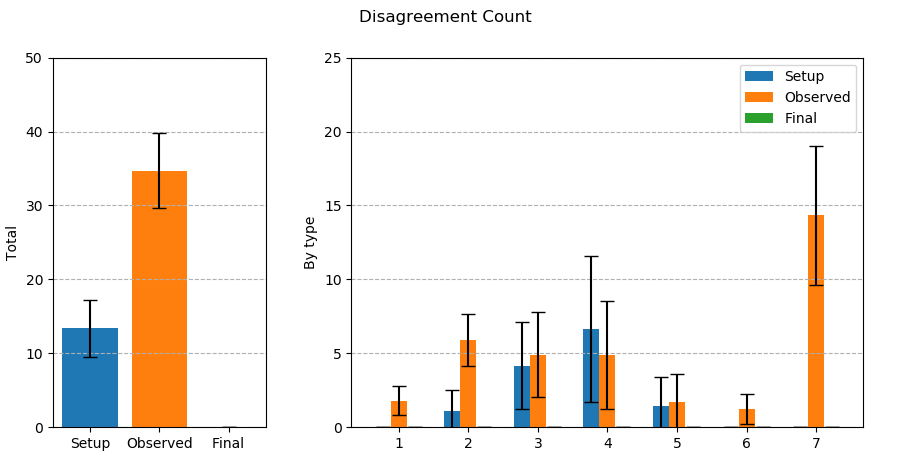
\includegraphics[width=\textwidth]{results/Figure_3_resized.png}
    \caption{The left plot presents the total count of disagreements, for all their types. On the right plot, the y-axis shows the  disagreement count for the types of disagreement displayed in the x-axis: 1.Self-Disagreement, 2.Overlap, 3. Hypo/hypernym, 4. Synonym, 5.Homonym, 6.Indistinguishable disagreement, 7.Untranslatable disagreement.}
    \label{fig:gen_count}
\end{figure}

In the left part of Figure \ref{fig:gen_count}, we can observe that the number of observed disagreements is more than twice the number of disagreements that have been set up. While disagreements spontaneously arise between two agents once they learned their first contrast sets over two different contexts, setting up disagreements increases the heterogeneity between the two agents' representations and causes a higher number of disagreements. The set up disagreements can be seen as ``stems'' for the observed disagreements. The final number of disagreements, which is counted after each argumentation, is always zero. This is not surprising, as an absence of disagreement is not necessarily equivalent to a full mutual agreement if the model admits a positive error threshold. The absence of overall disagreements is in fact the condition that tests the end of the argumentation between the agents in the systematic strategy, and therefore an equal-to-zero number of disagreements after the argumentation was expected.

The right part of Figure \ref{fig:gen_count} breaks down the count of disagreements for each different types of disagreements. As mentioned before, the only set up disagreement types that have a positive count are following: overlap,  hypo/hypernym,  synonym and the homonym. The distribution of the set up disagreements is directed by the cost of setting up each type: for instance, setting up an overlap requires three classes from the initial data set. On the other hand, setting up a synonymy only requires one class. Moreover, certain disagreements are causing other type of disagreements: for instance, setting up an overlap also sets up two hypo/hypernym disagreements.

The distribution of the observed disagreements is very different from the distribution of the setup disagreements. For instance, the most observed type of disagreement from the four types that are setup is the overlap disagreement, which was also the least set up type of disagreement. Indeed, since setting up an overlap requires to use 3 classes versus two at most for the other three types, they are expected to be less. The high incidence of overlap disagreements in the observed disagreements is an indicator that the overlap disagreement is the most likely to appear spontaneously when two agents learn their concepts over different contexts. Moreover, we can see that the most observed type of disagreements is the untranslatable disagreement. Since our error threshold is low ($\tau_{E} = 5)$, and since the Soybean data set has many small classes having about this number of examples, this is due to the agents over-fitting their intensional definitions because of the scarcity of examples in their initial data sets.


\begin{figure}
        \centering
        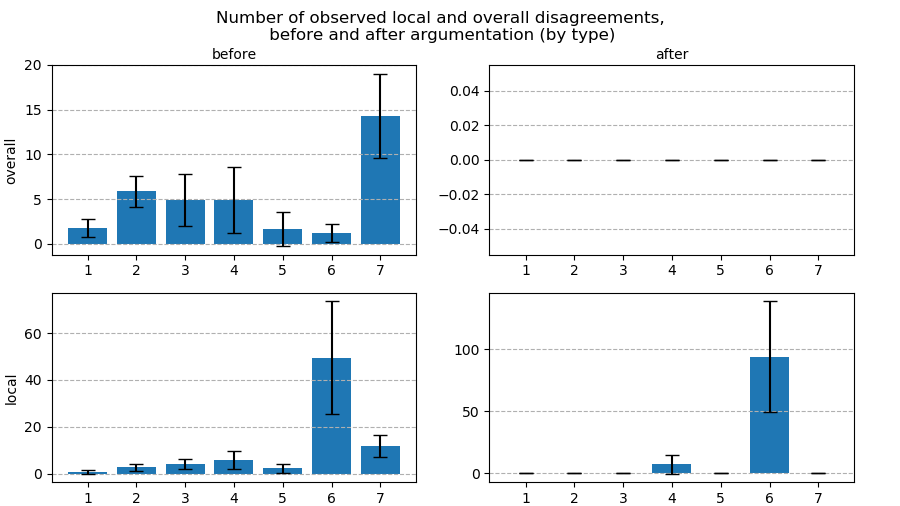
\includegraphics[width=\textwidth]{results/Figure_2_resized.png}
        \caption{The y-axis displays the count of each of the types of disagreement displayed in the x-axis: 1.Self-Disagreements, 2.Overlaps, 3. Hypo/hypernymies, 4. Synonymies, 5.Homonymies, 6.Indistinguishable disagreements, 7.Untranslatable disagreements}
        \label{fig:gen_local}
\end{figure}

Figure \ref{fig:gen_local} shows the count of each type of disagreements before and after the argumentation. The top figures represent the overall disagreements, while the bottom figures represent the local disagreements of one of the agent. Since the argumentation model is symmetrical and the disagreements are set up randomly, the other agent's counts follow a similar profile. On horizontal axis, the leftmost figures display the ODC, the disagreement count at the beginning of the argumentation, while the rightmost figures display the FDC, the disagreement count at the end of the argumentation. We can observe that while their are never overall disagreements after an argumentation, there are still local disagreements. While or model focuses on resolving every overall disagreements, it does not aim to resolve the local disagreements. Indeed, local disagreements do not necessarily stop the mutual intelligibility between the agents. Moreover, once there are no more overall disagreement between the agents anymore, eliminating the remaining local disagreements would require to exchange examples. While this would give more information to the agents, allowing them to observe directly that they have reached mutual intelligibility with their contexts, it would also go against our goal to keep the transfer of examples between the agents at the lowest possible amount.

\begin{figure}
    \centering
    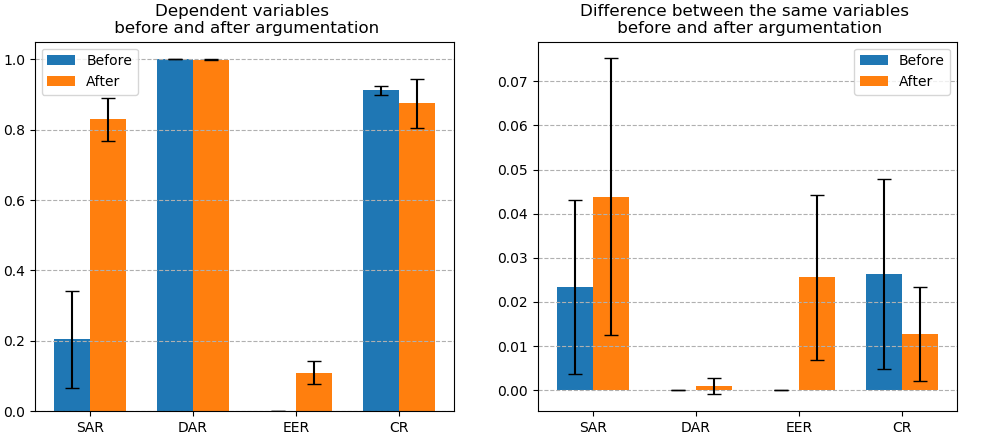
\includegraphics[width=\textwidth]{results/Figure_1_resized.png}
    \caption{}
    \label{fig:gen_intro}
\end{figure}

Figure \ref{fig:gen_intro} presents all the ratio that have been measured, before and after the argumentation. The most important are the SAR and the DAR, as the EER and the CR will be explored with more details in  future hypothesis tests. The leftmost figure presents the overall measures. The DAR, that is in essence a local measure which compares two contrast sets of a same agent, is here presented as the average of two DARs of the agents, averaged again over the 200 experiments. The rightmost figure presents the average difference between the local measures of a same experiment. Since the SAR, EER and CR are global measures, we propose a formulation for their local counterparts. The local SAR of an agent $A$ is computed by using the local context of $A$ instead of the overall context as the denominator of the ratio. The local EER of $A$ is computed by using the number of examples sent by $A$ as the numerator of the ratio, instead of using the number of examples exchanged by the two agents which would also include the number of examples received by $A$. Finally, the local CR of $A$ is computed by dividing the number of examples from $A$'s context that are covered by one of its current contrast set's concept, by the number of examples in $A$'s context.

We can see on the leftmost figure that the DAR of both agents is one both before and after the argumentation, meaning that the agents refined their respective contrast sets in a monotonic way, without compromising their original classifications. Moreover, the SAR significantly increases after the argumentation. The agents are therefore able to reach mutual intelligibility while refining their contrast sets in a monotonic way with our model. The EER stays around 0.1 with a low variance, meaning that the agents do not need to exchange more than $10\%$ of their examples to reach mutual intelligibility for any type of disagreement combination encountered. The CR decreases after the argumentation, meaning that less examples are covered after the argumentation. This is coherent with the fact that our model has been design to chose refinement over coverage. However, the difference between the CR before and after the argumentation is small, with a CR after argumentation well above 0.5, which indicates that the refinement does not cause an over-fitting.

The scale on the rightmost figure ranges from 0 to 0.08. This means that the difference between the local measures on the two agents ranges on a tenth of the global measures. From this, we can conclude that there is no asymmetry between the knowledge of our agents before or after the argumentation.

\subsection{Lazy Strategy}

%%% DOMAIN INDEPENDENCE
\section{Domain Independence}

The domain independence hypothesis postulates that both approaches of our model can resolve a disagreement between two agents that occurs on any domain, increasing the SAR of the agents while keeping their respective DAR at one. In order to test this hypothesis, we used with four different domains, and set up exactly \emph{one} overlap disagreement between two agents on each of them. Moreover, the examples that have not been used in the set up of the overlap are removed from the data set of the agents before the beginning of the argumentation, in order to ensure that we do not have more concepts that are not used in a set up in some domains than in others. We tested this experiment 100 times on and averaged the measures in order to present the results below. 

In each of the 100 experiments, the SAR, DAR, EEC and CR of the agents are measured in each of the four argumentation occurring on the different domains. The four domains are the independent variables our our experiment, while the SAR, DAR, EEC and CR are the dependent variables. The argument acceptability is 0.75, its standard value, and the redundancy is set at $0\%$ as usual. However, the error threshold is different for each data set. The error threshold is set in order to ensure that at least 3 classes from a set of classes of comparable sizes are available to set up the overlap in each data set. We decided on $\tau_{E} = 1$ for the Seat domain, $\tau_{E} = 6$ for the Zoology domain, $\tau_{E} = 10$ for the Sponges domain and $\tau_{E} = 11$ on the Soybean domain.

\subsection{Systematic Strategy}

\begin{figure}
    \centering
    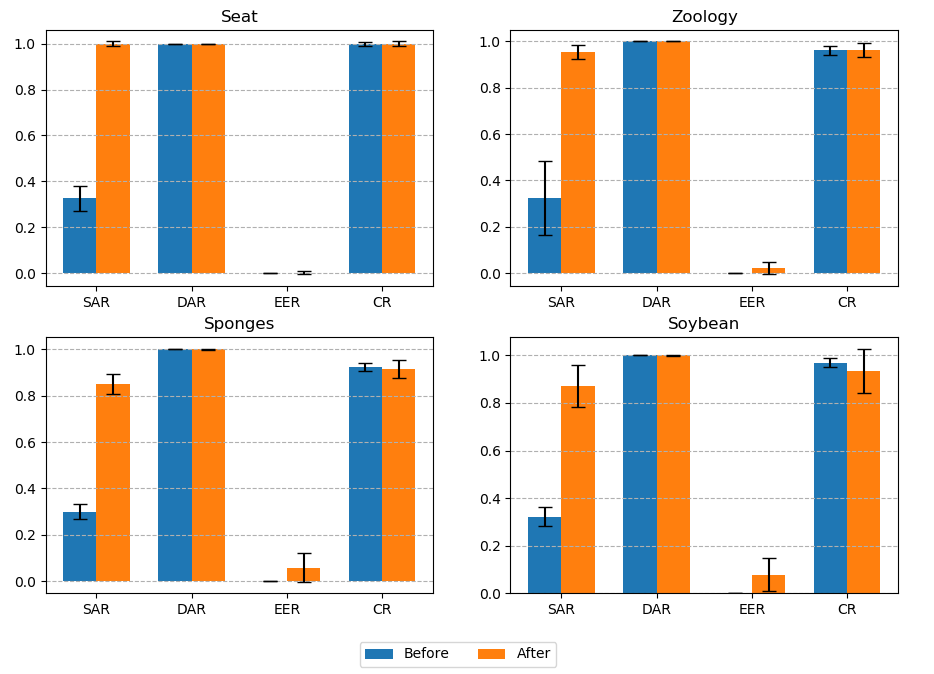
\includegraphics[width=\textwidth]{results/Figure_4_resized.png}
    \caption{Ratios measured before and after an argumentation, over the four different domains \emph{Seat}, \emph{Zoology}, \emph{Sponges} and \emph{Soybean}.}
    \label{fig:ind_intro}
\end{figure}

The results of this experiment are shown in Figure \ref{fig:ind_intro}. Each of the four sub-figures represents the four ratios measured on a specific domain, before and after the argumentation.
% SAR
We can observe a generalized increase of the SAR for all domains. The SAR before argumentation is on average at a predictable 0.33 for all domains, with a low variability except for the Zoology domain which is the domain where the distribution of the examples among the classes over $2 \times \tau_{E}$ elements is the most irregular. The average SAR after argumentation can vary from 0.83 to 1.0, depending on the domain. The systematic strategy achieves the highest increase of the SAR, with a final SAR of 1.0, meaning that the synchronic agreement is fully reached. The systematic strategy obtains a final SAR of 0.95 on average on the Zoology domain, and around 0.85 on the Sponges (0.85) and Soybean (0.87) domains. These results correlate with the complexity, in terms of different attributes, of the different domains.
% DAR
The DAR is maintained at 1 in every domain, with a standard deviation always close to 0. There is always a full diachronic agreement for both agents.

% EER
There are logically no example exchanged before the argumentation. The augmentations on the Seat domain are done without example exchanges, as the EER stays at 0 with a low standard deviation. On the other domains, the EER increases with the complexity of the domain expressed in terms of different attributes. Zoology accounts for the lowest non-zero EER, followed by Sponges and finally Soybean. The EER evolution is evaluated more in detail with the test of the preservation hypothesis.

% CR
The CRs before argumentation correlates on the complexity of the domain. The Seat domain has a CR at 1 with low standard deviation before the argumentation, the Zoology domain has a CR at 0.96, the Sponges has a CR at 0.92 and the Soybean has a CR at 0.97. The CR stays constant for the Seat and the Zoology domain. However, it decreases significantly for the Sponges add the Soybean domains, the decrease being more pronounced in the case of the Soybean domain. The decreases are again correlated to the complexity of the domains, however the final CR always stay close to the value it had before the argumentation. Even after the argumentation, every CR stays above 0.9, leaving the agents with less than $10\%$ of their overall context unclassified on average.

Overall, the performances of our model are high for every domain. The SAR is the most impacted measure by increments in the domain's complexity, with a lowest final SAR at 0.85 in the case of the Sponges domain and a highest final SAR at 1. The average final SAR being at 0.87 for the Soybean domain in this experiment, while it was at 0.83 in the last experiment, leads us to think that the average SAR measured in a situation of set up overlap is a good indicator of the SAR that should be expected for a combination of set up disagreements. The DAR remains at 1, proving once again to be the most stable measure.

\subsection{Lazy Strategy}

\section{Coverage Preservation}

The preservation hypothesis postulates that most of the examples that were covered by a concept continue to be covered by another concept in the refined contrast set. While a diachronic agreement ensures that no pair of examples from the same extensional definition \emph{of the new context} was separated in the initial contrast set, the diachronic agreement does not constraint the new context to be a super-set of the initial context. Therefore, as our model often refines concepts, we can expect that a context after an argumentation is a subset of itself before the argumentation. In this sense, the hypothesis of preservation complements the respect of the diachronic agreement in making sure that after an argumentation, an agent can make equivalent classifications as before \emph{over the same context}.

The preservation hypothesis has already been partially explored during the experiments over the Generality and Domain Independence hypotheses. However, the measures were approximated. Indeed, the overall CR computed was each time obtained as the average between both local CRs. This approximation is only accurate if one local set of covered examples is a subset of the other. In this section, the preservation hypothesis will be correctly investigated by searching for the subset of examples from the overall context that are not covered by \emph{both} agents. In order to evaluate this hypothesis over different contexts, we repeated this experiment 100 times on each domain over which we observed a final CR inferior to 1 during the test of the domain independence hypothesis: Zoology, Sponges and Soybean.

% VI & VD
The independent variables of each experiment and their overall set up are similar to the independent variables and set up of the domain independence hypothesis test. One argumentation is set up using three random classes of the selected domain. The domain is the only independent variable. The parameters are the same as for the domain independence hypothesis test. The dependent variables are however different: the overall CR is the only dependent variable observed, and it is this the ratio of the examples from the overall context subsumed by the intensional definition of at least one concept of each agent, by the size of the overall context.

\subsection{Systematic Strategy}

\subsection{Lazy Strategy}

\section{Efficiency}

In order to reach an agreement, the agents could transfer their entire contexts to each others. The issues of finding the overall pairing relations from the local ones and of creating new concepts through argumentation would disappear. The remaining tasks for our agents would only be to define new extensional definitions, learn satisfying intensional definitions for them and elect at new lexicon for the resulting contrast set. An important part of our model is dedicated to circumvent the problems arising when they cannot transfer these examples. The efficiency hypothesis proposes that the mutual intelligibility is not reached by the agents exchanging such extensively their contexts. In order to test this hypothesis over different contexts, we repeated this experiment 100 times on each domain over which we observed a non-zero EER during the test of the domain independence hypothesis: Zoology, Sponges and Soybean. 

% VI and VD
The independent variables of this experiment, its overall set up and its parameters are the same as for the test of the domain independence hypothesis. The dependent variables measured are the final overall EER, the difference between the two final local EERs, and the ratio of the final EER, by the SAR.

\subsection{Systematic Strategy}

\subsection{Lazy Strategy}

\section{Scalability}

The efficiency hypothesis questioned the ability of our model to reach mutual intelligibility while exchanging a reasonable amount of examples. The scalability hypothesis is its counterpart with generalizations. While we expect our model to exchange a number of generalizations significantly higher than the number of examples exchanged, the efficiency hypothesis investigates the correlation between the number of generalizations exchanged and the size of the overall context. Our hypothesis is that if the number of generalizations exchanged increases polynomially with the size of the overall context, therefore our model should be computally efficient once the size of the overall context reaches a certain threshold.

In order to test this hypothesis, we tested our argumentation with overall contexts of increasing sizes over the Sponge data set. The Sponge data set offers the advantage to have a larger version which enumerates 280 sponges, classified in the same three different orders ranging from 68 to 117 sponges. Our agents have an argumentation over a selected proportion of these 280 sponges ranging from 120 to 280, with the class distribution remaining the same for each proportion. This experiment is repeated 100 in order to present average results.

% VI & VD

\subsection{Systematic Strategy}

\subsection{Lazy Strategy}

\section{Simplicity}

In the introduction, we explained the difficulty to differentiate between hidden overlapping concepts that should be created, and small overlaps due to the agent's underfitting initial learning. However, while setting up the experiments, the number of concepts in the initial data set is known with certitude. Comparing this initial number with the final number of concepts present in the contrast sets \emph{after} the argumentation on meaning allows us to see how many excessive concepts have been created during the argumentation. However, this measure would be imperfect in the sense that it would penalize our model for something it is not directly aiming to solve: the precision of the agent's initial learning. As the argumentation on meaning takes place after the initial learning, the measure of simplicity should take into account \emph{all} the overlaps between the two contrast sets' concepts, which corresponds to the polylexematic classes of the union of the two agents' left-paths associations. By counting these polylexematic classes that contain more examples than the error threshold, we obtain the number of expected concepts (NEC). Comparing the NEC with the NFC (number of final concepts) gives us a measure of the simplicity of our model.

Our hypothesis of simplicity is that the average difference between the NEC and the NFC is close to 0. A difference above 0 would mean that our model converges by creating more concepts than necessary, which should increase the costs of our argumentation model in term of example and generalization exchanges. A difference below 0 would mean that our model creates less concepts than necessary, which should decrease either the synchronic agreement ratio or the coverage ratio. In order to evaluate this hypothesis over different contexts, we repeated the Domain Independence experiment 100 times on each domain over which we observed a final CR inferior to 1 during the test of the domain independence hypothesis: Zoology, Sponges and Soybean. Each time, we calculated the NEC and the NFC, subtracting the former to the latter. 

\subsection{Systematic Strategy}

\subsection{Lazy Strategy}

\section{Paradigm Shift}

We rationally demonstrated in the introduction that our model operates in a different paradigm than the AMAIL algorithm it was initially based on. This hypothesis of a paradigm shift in our argumentation model is also tested empirically. In order to evaluate this hypothesis, we test our model 100 times in the same conditions as we did for the Generality hypothesis, but this time running the AMAIL algorithm using the set of left-path associations of the agents before and after an argumentation with our model. We then compare the SAR, DAR and CR obtains at the two different times for each run. If there is indeed a paradigm shift, we should observe either a poor SAR, DAR, CR or no termination of the AMAIL algorithm at all before our argumentation, and an improved SAR but decreased DAR after our argumentation. 

\subsection{Systematic Strategy}

%% We compare the number of concepts in the original data set with the expected concepts at the creation of the contrast sets and the number of of concepts in output

% The VI are the domain, the number of concepts in the original data-set and the error threshold

% The VD are the the expected concepts at the creation of the contrast sets and the number of of concepts in output

% We do the same with the lazy strategy
\subsection{Lazy Strategy}